% Options for packages loaded elsewhere
% Options for packages loaded elsewhere
\PassOptionsToPackage{unicode}{hyperref}
\PassOptionsToPackage{hyphens}{url}
\PassOptionsToPackage{dvipsnames,svgnames,x11names}{xcolor}
%
\documentclass[
  11pt,
  a4paper]{article}
\usepackage{xcolor}
\usepackage[left=1in,top=1in,right=1in,bottom=1in]{geometry}
\usepackage{amsmath,amssymb}
\setcounter{secnumdepth}{-\maxdimen} % remove section numbering
\usepackage{iftex}
\ifPDFTeX
  \usepackage[T1]{fontenc}
  \usepackage[utf8]{inputenc}
  \usepackage{textcomp} % provide euro and other symbols
\else % if luatex or xetex
  \usepackage{unicode-math} % this also loads fontspec
  \defaultfontfeatures{Scale=MatchLowercase}
  \defaultfontfeatures[\rmfamily]{Ligatures=TeX,Scale=1}
\fi
\usepackage{lmodern}
\ifPDFTeX\else
  % xetex/luatex font selection
\fi
% Use upquote if available, for straight quotes in verbatim environments
\IfFileExists{upquote.sty}{\usepackage{upquote}}{}
\IfFileExists{microtype.sty}{% use microtype if available
  \usepackage[]{microtype}
  \UseMicrotypeSet[protrusion]{basicmath} % disable protrusion for tt fonts
}{}
\makeatletter
\@ifundefined{KOMAClassName}{% if non-KOMA class
  \IfFileExists{parskip.sty}{%
    \usepackage{parskip}
  }{% else
    \setlength{\parindent}{0pt}
    \setlength{\parskip}{6pt plus 2pt minus 1pt}}
}{% if KOMA class
  \KOMAoptions{parskip=half}}
\makeatother
% Make \paragraph and \subparagraph free-standing
\makeatletter
\ifx\paragraph\undefined\else
  \let\oldparagraph\paragraph
  \renewcommand{\paragraph}{
    \@ifstar
      \xxxParagraphStar
      \xxxParagraphNoStar
  }
  \newcommand{\xxxParagraphStar}[1]{\oldparagraph*{#1}\mbox{}}
  \newcommand{\xxxParagraphNoStar}[1]{\oldparagraph{#1}\mbox{}}
\fi
\ifx\subparagraph\undefined\else
  \let\oldsubparagraph\subparagraph
  \renewcommand{\subparagraph}{
    \@ifstar
      \xxxSubParagraphStar
      \xxxSubParagraphNoStar
  }
  \newcommand{\xxxSubParagraphStar}[1]{\oldsubparagraph*{#1}\mbox{}}
  \newcommand{\xxxSubParagraphNoStar}[1]{\oldsubparagraph{#1}\mbox{}}
\fi
\makeatother


\usepackage{longtable,booktabs,array}
\newcounter{none} % for unnumbered tables
\usepackage{calc} % for calculating minipage widths
% Correct order of tables after \paragraph or \subparagraph
\usepackage{etoolbox}
\makeatletter
\patchcmd\longtable{\par}{\if@noskipsec\mbox{}\fi\par}{}{}
\makeatother
% Allow footnotes in longtable head/foot
\IfFileExists{footnotehyper.sty}{\usepackage{footnotehyper}}{\usepackage{footnote}}
\makesavenoteenv{longtable}
\usepackage{graphicx}
\makeatletter
\newsavebox\pandoc@box
\newcommand*\pandocbounded[1]{% scales image to fit in text height/width
  \sbox\pandoc@box{#1}%
  \Gscale@div\@tempa{\textheight}{\dimexpr\ht\pandoc@box+\dp\pandoc@box\relax}%
  \Gscale@div\@tempb{\linewidth}{\wd\pandoc@box}%
  \ifdim\@tempb\p@<\@tempa\p@\let\@tempa\@tempb\fi% select the smaller of both
  \ifdim\@tempa\p@<\p@\scalebox{\@tempa}{\usebox\pandoc@box}%
  \else\usebox{\pandoc@box}%
  \fi%
}
% Set default figure placement to htbp
\def\fps@figure{htbp}
\makeatother





\setlength{\emergencystretch}{3em} % prevent overfull lines

\providecommand{\tightlist}{%
  \setlength{\itemsep}{0pt}\setlength{\parskip}{0pt}}



 


\usepackage{iftex}

% % Minion Pro
\usepackage[lf]{MinionPro}
\usepackage{MyriadPro}

% IBM Plex
% \usepackage{fontspec}
% \usepackage{unicode-math}
% \setmainfont{IBM Plex Serif}
% \setsansfont{IBM Plex Sans}
% \setmonofont{IBM Plex Mono}
% \setmathfont{IBM Plex Math Beta 240212}

% STIX Two
% \usepackage{fontspec}
% \setmainfont{Stix Two Text}
% \setmathfont{Stix Two Math}
% \setsansfont[Scale=0.9608140457]{Fira Sans} % 7.2489/7.54454

% Libertinus Serif + Libertinus Math + Source Sans Pro + Source Code Pro
% \ifPDFTeX
% \usepackage[mono=false,osf]{libertine}
% \usepackage[libertine]{newtxmath}
% % \usepackage[scale=1,osf]{sourcesanspro} % 7.1832/7.1832
% % \usepackage[scale=0.8772671637]{sourcecodepro} % 7.1832/7.36934*0.9
% \usepackage[scale=0.9181263229,osf]{roboto} % 7.1832/7.82376
% \usepackage[scale=0.8132241635]{roboto-mono} % 7.1832/7.94969*0.9
% \else
% \usepackage[mono=false,osf]{libertine}
% \setmathfont[Scale=MatchUppercase]{libertinusmath-regular.otf}
% % \usepackage[scale=0.9850312868,osf]{sourcesanspro} % 7.2051/7.31459
% % \usepackage[scale=0.8865281581]{sourcecodepro} % 7.2051/7.31459*0.9
% \usepackage[scale=0.9126225152,osf]{roboto} % 7.2051/7.89494
% \usepackage[scale=0.8213602637]{roboto-mono} % 7.2051/7.89494*0.9
% \fi

% Enable section and paragraph numbering
\setcounter{secnumdepth}{4} % Numbering down to paragraph level
\setcounter{tocdepth}{4} % Include paragraphs in the ToC

%%% CUSTOMIZE SECTION SIZES
\makeatletter
\renewcommand{\section}{%
  \@startsection{section}{1}
    {0pt} 					% indent
    {1.0em plus 0.2em minus 0.2em} 	% beforeskip
    {0.001em plus 0.001em minus 0.001em}    	% afterskip
    {\Large\bfseries\sffamily}%
}
\renewcommand{\subsection}{%
  \@startsection{subsection}{2}
    {0pt} 					% indent
    {1.0em plus 0.2em minus 0.2em} 	% beforeskip
    {0.001em plus 0.001em minus 0.001em}    	% afterskip
    {\large\bfseries\sffamily}%
}
\renewcommand{\subsubsection}{%
  \@startsection{subsubsection}{3}
    {0pt} 					% indent
    {1.0em plus 0.2em minus 0.2em} 	% beforeskip
    {0.001em plus 0.001em minus 0.001em}    	% afterskip
    {\normalsize\bfseries\sffamily}%
}
\renewcommand{\paragraph}{%
  \@startsection{paragraph}{4}
    {0pt} 					% indent
    {1.0em plus 0.2em minus 0.2em} 	% beforeskip
    {0.001em plus 0.001em minus 0.001em}    	% afterskip
    {\normalsize\bfseries\sffamily}%
}
\makeatother

%%% GENERAL PACKAGES
\usepackage{hyphenat} % don't hyphenat titles
\usepackage{graphicx}
\usepackage{tabularx} 
\usepackage{marvosym} % Mail logo
\usepackage{enumitem} % Enumerate items (list)
\usepackage{amsmath} % for enhanced math features
\usepackage[labelfont=bf,justification=justified,singlelinecheck=false]{caption} % Figures caption setup
\usepackage[rightcaption]{sidecap} % figure with sidecaption
\usepackage[]{lineno} % Line numbers
\usepackage{ragged2e} % justify
\usepackage{array}
\usepackage{lscape} % landscape tables
\usepackage{rotating} % landscape tables
\usepackage{bm} % bold math

%%%% ORCID LOGO
\usepackage{academicons}
\definecolor{orcidlogocol}{HTML}{A6CE39}
\usepackage{orcidlink}

%%%% LAYOUT 
\tolerance=200
\emergencystretch=2em
\hyphenpenalty=1000
\hbadness=2000
\widowpenalty=1000 % widow penalty
\clubpenalty=1000 % orphans penalty
\renewcommand{\baselinestretch}{1.3333333333333333333333333333} % line spacing

\renewcommand{\arraystretch}{1.3333}
\makeatletter
\@ifpackageloaded{float}{}{\usepackage{float}}
\floatstyle{plain}
\@ifundefined{c@chapter}{\newfloat{suppfig}{h}{losuppfig}}{\newfloat{suppfig}{h}{losuppfig}[chapter]}
\floatname{suppfig}{Figure S}
\newcommand*\quartosuppfigref[1]{Figure \hyperref[#1]{S\ref{#1}}}
\@ifpackageloaded{caption}{}{\usepackage{caption}}
\DeclareCaptionLabelFormat{quartosuppfigreflabelformat}{#1#2}
\captionsetup[suppfig]{labelformat=quartosuppfigreflabelformat}
\newcommand*\listofsuppfigs{\listof{suppfig}{List of Supplementary Figures}}
\makeatother
\makeatletter
\@ifpackageloaded{float}{}{\usepackage{float}}
\floatstyle{plain}
\@ifundefined{c@chapter}{\newfloat{supptbl}{h}{losupptbl}}{\newfloat{supptbl}{h}{losupptbl}[chapter]}
\floatname{supptbl}{Table S}
\floatstyle{plaintop}
\restylefloat{supptbl}
\newcommand*\quartosupptblref[1]{Table \hyperref[#1]{S\ref{#1}}}
\@ifpackageloaded{caption}{}{\usepackage{caption}}
\DeclareCaptionLabelFormat{quartosupptblreflabelformat}{#1#2}
\captionsetup[supptbl]{labelformat=quartosupptblreflabelformat}
\newcommand*\listofsupptbls{\listof{supptbl}{List of Supplementary Tables}}
\makeatother
\makeatletter
\@ifpackageloaded{caption}{}{\usepackage{caption}}
\AtBeginDocument{%
\ifdefined\contentsname
  \renewcommand*\contentsname{Table of contents}
\else
  \newcommand\contentsname{Table of contents}
\fi
\ifdefined\listfigurename
  \renewcommand*\listfigurename{List of Figures}
\else
  \newcommand\listfigurename{List of Figures}
\fi
\ifdefined\listtablename
  \renewcommand*\listtablename{List of Tables}
\else
  \newcommand\listtablename{List of Tables}
\fi
\ifdefined\figurename
  \renewcommand*\figurename{Figure}
\else
  \newcommand\figurename{Figure}
\fi
\ifdefined\tablename
  \renewcommand*\tablename{Table}
\else
  \newcommand\tablename{Table}
\fi
}
\@ifpackageloaded{float}{}{\usepackage{float}}
\floatstyle{ruled}
\@ifundefined{c@chapter}{\newfloat{codelisting}{h}{lop}}{\newfloat{codelisting}{h}{lop}[chapter]}
\floatname{codelisting}{Listing}
\newcommand*\listoflistings{\listof{codelisting}{List of Listings}}
\makeatother
\makeatletter
\makeatother
\makeatletter
\@ifpackageloaded{caption}{}{\usepackage{caption}}
\@ifpackageloaded{subcaption}{}{\usepackage{subcaption}}
\makeatother
\usepackage{bookmark}
\IfFileExists{xurl.sty}{\usepackage{xurl}}{} % add URL line breaks if available
\urlstyle{same}
\hypersetup{
  pdftitle={Mechanical power output during stretch--shortening cycles of rat medial gastrocnemius muscle: influence of various muscle length trajectories -- S3 File},
  colorlinks=true,
  linkcolor={blue},
  filecolor={Maroon},
  citecolor={Blue},
  urlcolor={Blue},
  pdfcreator={LaTeX via pandoc}}


\title{Mechanical power output during stretch--shortening cycles of rat
medial gastrocnemius muscle: influence of various muscle length
trajectories -- S3 File}
\author{}
\date{}
\begin{document}


\linenumbers

\renewcommand{\thesection}{S\arabic{section}}
\setcounter{section}{2}
\floatname{suppfig}{Figure }
\renewcommand{\thesuppfig}{\thesection.\arabic{suppfig}}
\renewcommand*\quartosuppfigref[1]{Figure~\ref{#1}}

\phantomsection

\section{Optimal CE length over time: influence of FTS and MTC length
excursion}\label{optimal-ce-length-over-time-influence-of-fts-and-mtc-length-excursion}

Using the Hill-type MTC model, we identified the optimal CE length over
time for maximal AMPO without imposing any constraints on MTC length
over time. When imposing cycle frequency, the resulting MTC length over
time was reasonably similar to that with constant MTC shortening and
lengthening velocity. However, when imposing FTS or MTC length excursion
the shape of CE and MTC length over time dramatically changed.

For imposed FTS values below the optimal value, CE lengthening velocity
was found to be almost zero at the onset of CE lengthening
(\quartosuppfigref{suppfig-s-oc}A). This infinitely low velocity at the
start of CE lengthening was optimal for AMPO because it allowed the
active state to decrease fully before lengthening occurred, thereby
reducing the amount of negative mechanical work performed. On top of
that, it allowed the active state to remain high throughout most part of
CE shortening to enable substantial positive mechanical work. Towards
the end of CE lengthening, CE velocity again approached zero, which made
it possible to initiate muscle stimulation before CE shortening began.
This resulted in a high active state at the onset of CE shortening to
enhance positive mechanical work. For imposed FTS values above the
optimal value, CE shortening velocity decreased over time at the end of
CE shortening (\quartosuppfigref{suppfig-s-oc}A). To avoid substantial
negative mechanical work during the subsequent CE lengthening, muscle
stimulation ceased well before the end of CE shortening. While CE could
theoretically maintain a constant shortening velocity throughout the
shortening phase, any additional positive mechanical work gained near
the end was outweighed by the increased negative mechanical work. Thus,
an almost isometric phase preceding CE lengthening is optimal for
maximising AMPO. In sum, the CE length over time for imposed FTS values
mostly results from the effect of the excitation dynamics.

For imposed MTC length excursions above the optimal value, CE shortening
velocity was found to be higher at the beginning and end of the
shortening phase compared to the middle part
(\quartosuppfigref{suppfig-s-oc}B). At the start and end of the
shortening phase, only limited positive mechanical work could be
produced due to the low active state and the suboptimal CE length (that
is due to the CE force-length relationship). While CE could
theoretically shorten at a constant velocity throughout the entire
shortening phase, this would reduce the positive mechanical work during
the middle part due to the effect of the force-velocity relationship. At
the same time, little additional positive mechanical work could be
achieved at the beginning and end of the shortening phase (due to the
low active state and suboptimal CE length). Consequently, a non-constant
CE shortening velocity --- with CE shortening first decreasing and then
increasing during the shortening phase --- is optimal for maximising
AMPO at imposed MTC length excursions above the optimal value. For
imposed MTC length excursions below the optimal value, the opposite
pattern was found: CE shortening velocity was found to be lower at the
beginning and end of the shortening phase compared to the middle part
(\quartosuppfigref{suppfig-s-oc}B). As explained, only limited positive
mechanical work could be produced at the beginning and end of the
shortening phase due to the low active state. If CE would shorten with a
constant velocity throughout the entire shortening phase, this would
decrease the shortening distance during the middle part (at which the
active state is high) and thereby reduces the positive mechanical work.
As a result, a non-constant CE shortening velocity --- with a slow
shortening velocity at the end and beginning of the shortening phase ---
is optimal for maximising AMPO at imposed MTC length excursions above
the optimal value. In sum, the optimal CE length over time for imposed
MTC length excursions shows the intricate trade-off between the CE
force-length relationship, CE force-velocity relationship and the
excitation dynamics.

\begin{suppfig}

\centering{

\pandocbounded{
\includegraphics[keepaspectratio]{../figures/s_oc.pdf}}

}

\caption{\label{suppfig-s-oc}\textbf{Predicted CE length over time for
maximally attainable AMPO, shown for two imposed FTS values (A) and two
imposed MTC length excursions (B), at a cycle frequency of 3.5 Hz for
rat 1}. In panel A, only cycle frequency and FTS were imposed, while in
panel B only cycle frequency and MTC length excursions were imposed.
Apart from these two constraints, CE and MTC length over time were
completely unconstrained and thus the shape of CE length over time could
be different between every combination of imposed cycle frequency and
FTS (A) or imposed cycle frequency and MTC length excursion (B). CE
stimulation was maximal during the period indicated by the coloured
bars, and `off' elsewhere.}

\end{suppfig}%

\begin{suppfig}

\centering{

\pandocbounded{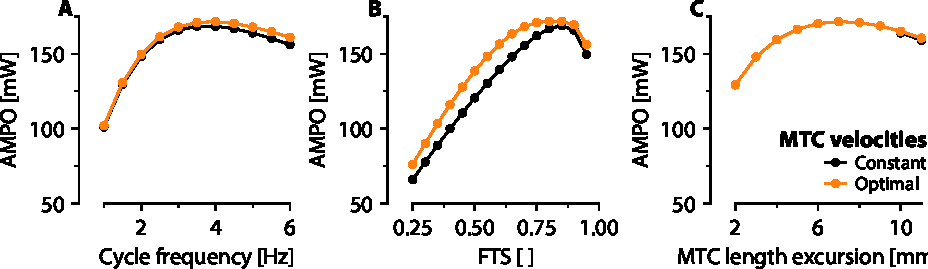
\includegraphics[keepaspectratio]{../figures/s_ampo.pdf}}

}

\caption{\label{suppfig-s-ampo}\textbf{Predicted influence of cycle
frequency (A), FTS (B) and MTC length excursion (C) on the maximum
attainable AMPO}. The maximally attainable AMPO --- averaged across the
three rats --- slightly increased in SSCs without a constraint on MTC
length over time (orange lines), compared to SSCs with a constant MTC
shortening and lengthening velocity (black lines).}

\end{suppfig}%




\end{document}
